\documentclass[12pt, oneside]{article}

\usepackage[letterpaper, scale=0.89, centering]{geometry}
\usepackage{fancyhdr}
\setlength{\parindent}{0em}
\setlength{\parskip}{1em}

\pagestyle{fancy}
\fancyhf{}
\renewcommand{\headrulewidth}{0pt}
\rfoot{\href{https://creativecommons.org/licenses/by-nc-sa/2.0/}{CC BY-NC-SA 2.0} Version \today~(\thepage)}

\usepackage{amssymb,amsmath,pifont,amsfonts,comment,enumerate,enumitem}
\usepackage{currfile,xstring,hyperref,tabularx,graphicx,wasysym}
\usepackage[labelformat=empty]{caption}
\usepackage[dvipsnames,table]{xcolor}
\usepackage{multicol,multirow,array,listings,tabularx,lastpage,textcomp,booktabs}

\lstnewenvironment{algorithm}[1][] {   
    \lstset{ mathescape=true,
        frame=tB,
        numbers=left, 
        numberstyle=\tiny,
        basicstyle=\rmfamily\scriptsize, 
        keywordstyle=\color{black}\bfseries,
        keywords={,procedure, div, for, to, input, output, return, datatype, function, in, if, else, foreach, while, begin, end, }
        numbers=left,
        xleftmargin=.04\textwidth,
        #1
    }
}
{}
\lstnewenvironment{java}[1][]
{   
    \lstset{
        language=java,
        mathescape=true,
        frame=tB,
        numbers=left, 
        numberstyle=\tiny,
        basicstyle=\ttfamily\scriptsize, 
        keywordstyle=\color{black}\bfseries,
        keywords={, int, double, for, return, if, else, while, }
        numbers=left,
        xleftmargin=.04\textwidth,
        #1
    }
}
{}

\newcommand\abs[1]{\lvert~#1~\rvert}
\newcommand{\st}{\mid}

\newcommand{\A}[0]{\texttt{A}}
\newcommand{\C}[0]{\texttt{C}}
\newcommand{\G}[0]{\texttt{G}}
\newcommand{\U}[0]{\texttt{U}}

\newcommand{\cmark}{\ding{51}}
\newcommand{\xmark}{\ding{55}}
 
\begin{document}
\begin{flushright}
    \StrBefore{\currfilename}{.}
\end{flushright} \section*{Week8 monday}



{\bf  Theorem}: $A_{TM}$  is  not  Turing-decidable.

{\bf  Proof}: Suppose {\bf towards a  contradiction}  that there  is a Turing machine  that decides $A_{TM}$.  
We call this presumed machine  $M_{ATM}$.

By  assumption, for every  Turing machine  $M$ and every  string $w$

\begin{itemize}
\item If $w \in L(M)$, then  the computation of $M_{ATM}$  on  $\langle M,w \rangle ~~ \underline{\phantom{\hspace{2.5in}}}$
\item If $w \notin L(M)$, then  the computation of $M_{ATM}$  on  $\langle M,w \rangle ~~ \underline{\phantom{\hspace{2.5in}}}$
\end{itemize}


Define  a {\bf new} Turing machine using  the high-level description:
\begin{quote}
$D =  $`` On  input $\langle M \rangle$, where  $M$  is  a Turing machine:
\begin{itemize}
\item[1.] Run  $M_{ATM}$ on  $\langle M, \langle M \rangle  \rangle$.
\item[2.] If $M_{ATM}$ accepts, reject; if  $M_{ATM}$ rejects, accept."
\end{itemize}
\end{quote}


Is $D$ a  Turing machine?

\vspace{50pt}

Is  $D$ a  decider? 

\vspace{50pt}

What is the result of the computation  of $D$  on  $\langle D \rangle$?

\vfill

\newpage

{\bf  Theorem} (Sipser Theorem 4.22): A  language is Turing-decidable if and only if both  it and its complement
are Turing-recognizable.

{\bf Proof, first direction:}  Suppose  language  $L$ is  Turing-decidable.   WTS  that both it and its complement 
are Turing-recognizable.

\vfill

{\bf Proof, second direction:}  Suppose  language  $L$ is  Turing-recognizable, and  so is  its complement.   WTS  that $L$
is Turing-decidable.
\vfill


Give an example of a {\bf decidable} set: 

\vspace{20pt}

Give an example of a {\bf recognizable undecidable} set: 

\vspace{20pt}

Give an example of an {\bf unrecognizable} set: 

\vspace{20pt}


\newpage

{\bf True} or {\bf False}: The class of Turing-decidable languages is closed under complementation?

\vfill
\vfill
\vfill
Definition: A language $L$ over an  alphabet $\Sigma$ is called {\bf co-recognizable} if its complement,  defined
as $\Sigma^* \setminus L  = \{ x  \in  \Sigma^* \mid x \notin  L \}$, is Turing-recognizable.


Notation: The complement  of a set $X$ is denoted with  a superscript $c$, $X^c$, or an overline,  $\overline{X}$.
 \vfill
\section*{Week8 wednesday}


{\bf Mapping reduction}

Motivation: Proving that $A_{TM}$ is undecidable was hard. How can we leverage that work? 
Can we relate the decidability / undecidability of one problem to another?

\begin{quote}
If problem $X$ is {\bf no harder than} problem $Y$

\ldots and if $Y$ is easy,

\ldots then $X$ must be easy too.
\end{quote}


\begin{quote}
    If problem $X$ is {\bf no harder than} problem $Y$
    
    \ldots and if $X$ is hard,
    
    \ldots then $Y$ must be hard too.
\end{quote}

``Problem $X$ is no harder than problem $Y$'' means 
``Can answer questions about membership in $X$ by converting them to questions about membership in $Y$''.



Definition:  $A$ is  {\bf  mapping  reducible to} $B$  means there is a computable function 
$f : \Sigma^* \to \Sigma^*$ such that {\it for all} strings  $x$ in $\Sigma^*$, 
\[
x  \in  A \qquad \qquad \text{if and  only  if} \qquad \qquad f(x) \in B.
\]
Notation:  when $A$  is mapping reducible to $B$, we write $A  \leq_m B$.

{\it Intuition:} $A \leq_m B$ means $A$ is no harder than $B$, i.e. that the level 
of difficulty of $A$ is less than or equal the level of difficulty of $B$.

\vfill

\newpage
{\bf Computable functions}

Definition: A function $f: \Sigma^* \to \Sigma^*$ is a {\bf computable function} means there is some Turing machine such that, 
for each $x$, on input $x$ the Turing machine halts with exactly $f(x)$ followed by all blanks on the tape

{\it Examples of computable functions}:

The function that maps a string to a string which is one character longer and 
whose value, when interpreted as a fixed-width binary representation of a
nonnegative integer is twice the value of the input string (when interpreted as 
a fixed-width binary representation of a non-negative integer)
\[
f_1: \Sigma^* \to \Sigma^* \qquad  f_1(x)  = x0
\]

To prove $f_1$ is computable function, we define a Turing machine computing it.

{\it High-level description}
\begin{quote}
    ``On input $w$
    
    1. Append $0$ to $w$.
    
    2. Halt.''
\end{quote}

{\it Implementation-level description}
\begin{quote}
    ``On input $w$
    
    1. Sweep read-write head to the right until find first blank cell.
    
    2. Write 0.
    
    3. Halt.''
\end{quote}

{\it Formal definition} $(\{q0, qacc, qrej\}, \{0,1\}, \{0,1,\textvisiblespace\},\delta, q0, qacc, qrej)$
where $\delta$ is specified by the state diagram: 


\newpage


The function that maps a string to the result of repeating the string twice.
\[
f_2: \Sigma^* \to \Sigma^* \qquad f_2( x )  =  xx
\]

\vfill

The function that maps strings that are not the codes of Turing machines to the empty 
string and that maps strings that code Turing machines to the code of the 
related Turing machine that acts like the Turing machine coded by the input, except
that if this Turing machine coded by the input tries to reject, the 
new machine will go into a loop.
\[
f_3: \Sigma^* \to \Sigma^*  \qquad f_3( x )  =   \begin{cases}  \varepsilon \qquad&\text{if $x$ is not the code of  a TM} \\
\langle (Q \cup \{q_{trap} \}, \Sigma, \Gamma, \delta', q_0, q_{acc}, q_{rej} ) \rangle \qquad&\text{if $x = \langle (Q, \Sigma, \Gamma, \delta, q_0, q_{acc}, q_{rej} )\rangle$}\end{cases}
\]
where $q_{trap} \notin Q$ and 
\[\delta'( (q,x) ) = \begin{cases}
(r,y,d) &\text{if $q \in Q$, $x \in \Gamma$, $\delta ((q,x)) = (r,y,d)$, and  $r \neq  q_{rej}$} \\
(q_{trap}, \textvisiblespace, R) & \text{otherwise}
\end{cases}
\]
\vfill

\newpage


The function that maps strings that are not the codes of CFGs to the empty 
string and that maps strings that code CFGs to the code of a PDA that recognizes
the language generated by the CFG.


\vfill

{\it Other examples?}
 \vfill
\section*{Week8 friday}



Recall definition:  $A$ is  {\bf  mapping  reducible to} $B$  means there is a computable function 
$f : \Sigma^* \to \Sigma^*$ such that {\it for all} strings  $x$ in $\Sigma^*$, 
\[
x  \in  A \qquad \qquad \text{if and  only  if} \qquad \qquad f(x) \in B.
\]
Notation:  when $A$  is mapping reducible to $B$, we write $A  \leq_m B$.

{\it Intuition:} $A \leq_m B$ means $A$ is no harder than $B$, i.e. that the level 
of difficulty of $A$ is less than or equal the level of difficulty of $B$.


{\it Example}: $A_{TM} \leq_m A_{TM}$ 

\vfill

{\it Example}: $A_{DFA} \leq_m \{ ww \mid  w \in \{0,1\}^* \}$ 

\vfill



{\it Example}: $\{ 0^i  1^j \mid i  \geq 0, j \geq 0 \} \leq_m A_{TM}$ 

\vfill

{\bf Theorem} (Sipser 5.22): If $A \leq_m B$ and $B$ is decidable, then $A$ is decidable.
    

{\bf Theorem} (Sipser 5.23): If $A \leq_m B$ and $A$ is undecidable, then $B$ is undecidable.
    

\newpage

    {\bf Halting problem}
    \[
    HALT_{TM} = \{ \langle M, w \rangle \mid \text{$M$ is a  Turing machine, $w$ is  a string, and $M$ halts on $w$} \}
    \]
    
    Define $F: \Sigma^* \to \Sigma^*$ by
    \[
    F(x) =  \begin{cases}
    const_{out} \qquad &\text{if  $x \neq \langle M,w \rangle$ for any Turing machine  $M$ and string  $w$ over the alphabet of $M$} \\
    \langle M', w \rangle \qquad &  \text{if $x = \langle M, w \rangle$ for some Turing machine  $M$ and string $w$ over the alphabet of $M$.}
    \end{cases}
    \]
    where $const_{out}  =  \langle  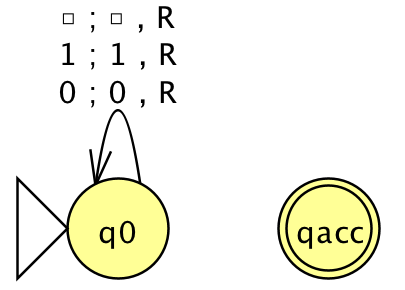
\includegraphics[width=1.5in]{resources/machines/Lect22TM1.png} ,  \varepsilon  \rangle$
    and  $M'$ is a Turing machine that computes like $M$ except, if the computation ever were to go to a  reject state,
    $M'$ loops instead.
    
    \vfill

    $F( \langle 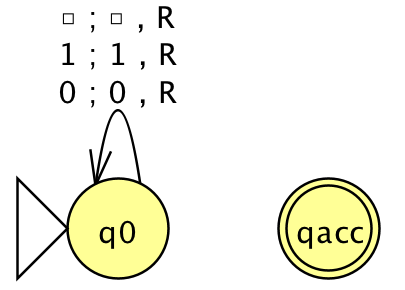
\includegraphics[width=1.5in]{resources/machines/Lect22TM1.png} ,  001  \rangle)$ =

    \vfill

    $F( \langle 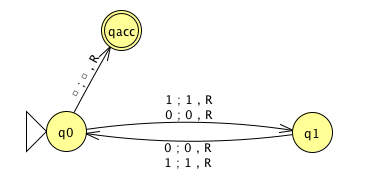
\includegraphics[width=2.5in]{resources/machines/Lect22TM2.png} ,  1  \rangle)$ =

    \vfill
    
    \newpage
    To use this function  to prove that $A_{TM} \leq_m HALT_{TM}$, we need  two claims:

    
    Claim (1): $F$ is computable \phantom{\hspace{2in}}
    
    \vfill

    Claim (2): for every  $x$,  $x \in  A_{TM}$ iff $F(x) \in HALT_{TM}$.  
    
    \vfill
     \vfill
\section*{Week7 monday}



\begin{center}
    \begin{tabular}{|l|l|l|l|}
    \hline
    & Suppose $M$ is  a TM & Suppose $D$ is  a TM & Suppose $E$ is  an
    enumerator  \\
    &that  recognizes $L$  &that  decides $L$  &that enumerates $L$ \\
    \hline
    If string $w$ is in  $L$ then  \ldots  &&& \\
    &&&\\
    &&&\\
    If string $w$ is not in  $L$ then  \ldots  && &\\
    &&&\\
    &&&\\
    \hline
    \end{tabular}
\end{center}
    
    {\bf Describing  Turing machines} (Sipser p. 185)
    
    The Church-Turing thesis posits that each algorithm can be implemented by some Turing machine

    High-level descriptions of  Turing machine algorithms are written as indented text within quotation marks.   

    Stages of the algorithm are typically numbered consecutively.

    The first line specifies the input to the machine, which must be a string.
    This string may be the encoding of some object or  list of  objects.  
    
    {\bf Notation:} $\langle O \rangle$ is the string that encodes the object $O$.
    $\langle O_1, \ldots, O_n \rangle$ is the string that encodes the list of objects $O_1, \ldots, O_n$.
    
    {\bf Assumption}: There are Turing  machines that can be called as subroutines
    to decode the string representations of common objects and  interact with these objects as intended
    (data structures).
    
    \newpage    
    For example, since there are algorithms to answer each of the following questions,
    by Church-Turing thesis, there is a Turing machine that accepts exactly those strings for which the 
    answer to the question is ``yes''
    \begin{itemize}
        \item Does a string over $\{0,1\}$ have even length?

        \vfill

        \item Does a string over $\{0,1\}$ encode a string of ASCII characters?\footnote{An introduction to ASCII 
        is available on the w3 tutorial \href{https://www.w3schools.com/charsets/ref_html_ascii.asp}{here}.}

        \vfill

        \item Does a DFA have a specific number of states?

        \vfill

        \item Do two NFAs have any state names in common?

        \vfill

        \item Do two CFGs have the same start variable?

        \vfill

      \end{itemize}

\newpage

A {\bf computational problem} is decidable iff language encoding its positive problem instances
is decidable.

The computational problem ``Does a specific DFA accept a given string?'' is encoded by the language
\begin{align*}
  &\{ \textrm{representations of DFAs $M$ and strings $w$ such that $w \in L(M)$}\}  \\
  =& \{ \langle M, w \rangle \mid M \textrm{ is a DFA}, w \textrm{ is a string}, w \in L(M) \}
\end{align*}

The computational problem ``Is the language generated by a CFG empty?'' is encoded by the language
\begin{align*}
  &\{ \textrm{representations of CFGs $G$  such that $L(G) = \emptyset$}\}  \\
  =& \{ \langle G \rangle \mid G \textrm{ is a CFG},  L(G) = \emptyset \}
\end{align*}



The computational problem ``Is the given Turing machine a decider?'' is encoded by the language
\begin{align*}
  &\{ \textrm{representations of TMs $M$  such that $M$ halts on every input}\}  \\
  =& \{ \langle M \rangle \mid M \textrm{ is a TM and for each string } w, \textrm{$M$ halts on $w$} \}
\end{align*}


{\it Note: writing down the language encoding a computational problem is only the first step in 
determining if it's recognizable, decidable, or \ldots }


{\bf Some classes of computational problems help us understand the differences between the machine models we've been studying:}

\vspace{-20pt}

    \begin{center}
    \begin{tabular}{|lcl|}
    \hline
    \multicolumn{3}{|l|}{{\bf  Acceptance problem} } \\
    & & \\
    \ldots for DFA & $A_{DFA}$ & $\{ \langle B,w \rangle \mid  \text{$B$ is a  DFA that accepts input 
    string $w$}\}$ \\
    \ldots for NFA & $A_{NFA}$ & $\{ \langle B,w \rangle \mid  \text{$B$ is a  NFA that accepts input 
    string $w$}\}$ \\
    \ldots for regular expressions & $A_{REX}$ & $\{ \langle R,w \rangle \mid  \text{$R$ is a  regular
    expression that generates input string $w$}\}$ \\
    \ldots for CFG & $A_{CFG}$ & $\{ \langle G,w \rangle \mid  \text{$G$ is a context-free grammar 
    that generates input string $w$}\}$ \\
    \ldots for PDA & $A_{PDA}$ & $\{ \langle B,w \rangle \mid  \text{$B$ is a PDA that accepts input string $w$}\}$ \\
    & & \\
    & & \\
    \hline
    \multicolumn{3}{|l|}{{\bf Language emptiness  testing} } \\
    & & \\
    \ldots for DFA & $E_{DFA}$ & $\{ \langle A \rangle \mid  \text{$A$ is a  DFA and  $L(A) = \emptyset$\}}$ \\
    \ldots for NFA & $E_{NFA}$ & $\{ \langle A\rangle \mid  \text{$A$ is a NFA and  $L(A) = \emptyset$\}}$ \\
    \ldots for regular expressions & $E_{REX}$ & $\{ \langle R \rangle \mid  \text{$R$ is a  regular
    expression and  $L(R) = \emptyset$\}}$ \\
    \ldots for CFG & $E_{CFG}$ & $\{ \langle G \rangle \mid  \text{$G$ is a context-free grammar 
    and  $L(G) = \emptyset$\}}$ \\
    \ldots for PDA & $E_{PDA}$ & $\{ \langle A \rangle \mid  \text{$A$ is a PDA and  $L(A) = \emptyset$\}}$ \\
    & & \\
    & & \\
    \hline
    \multicolumn{3}{|l|}{{\bf Language equality testing} } \\
    & & \\
    \ldots for DFA & $EQ_{DFA}$ & $\{ \langle A, B \rangle \mid  \text{$A$ and $B$ are DFAs and  $L(A) =L(B)$\}}$\\
    \ldots for NFA & $EQ_{NFA}$ & $\{ \langle A, B \rangle \mid  \text{$A$ and $B$ are NFAs and  $L(A) =L(B)$\}}$\\
    \ldots for regular expressions & $EQ_{REX}$ & $\{ \langle R, R' \rangle \mid  \text{$R$ and $R'$ are regular
    expressions and  $L(R) =L(R')$\}}$\\
    \ldots for CFG & $EQ_{CFG}$ & $\{ \langle G, G' \rangle \mid  \text{$G$ and $G'$ are CFGs and  $L(G) =L(G')$\}}$ \\
    \ldots for PDA & $EQ_{PDA}$ & $\{ \langle A, B \rangle \mid  \text{$A$ and $B$ are PDAs and  $L(A) =L(B)$\}}$ \\
    \hline
    Sipser Section 4.1 &&\\
    \hline
    \end{tabular}
    \end{center}
    
    
    
    \newpage
    
    \begin{center}
    \begin{tabular}{|c|c|c|}
    \hline
    $M_1$  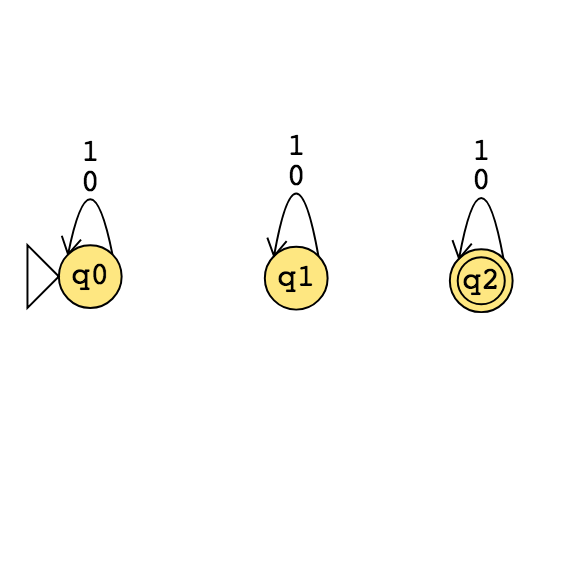
\includegraphics[width=2in]{resources/machines/Lect17DFA1.png} &  
    $M_2$ 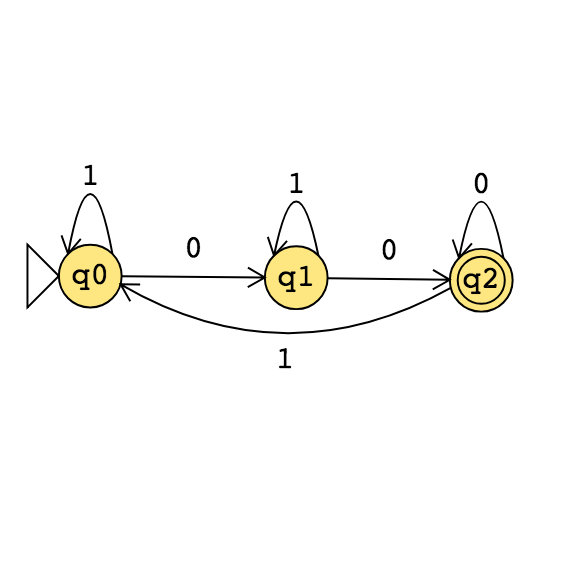
\includegraphics[width=2in]{resources/machines/Lect17DFA2.png} &  
    $M_3$ 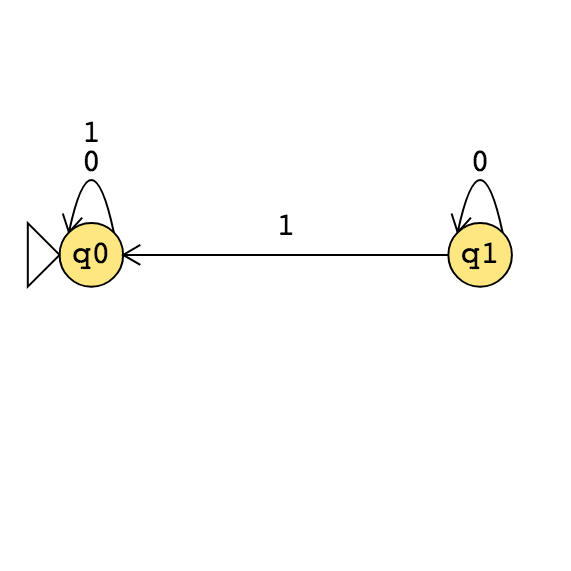
\includegraphics[width=2in]{resources/machines/Lect17DFA3.png} \\ 
    && \\
    && \\
    && \\
    && \\
    \hline
    \end{tabular}
    \end{center}
    
    Example strings in $A_{DFA}$
    
    \vfill
    
    Example strings in  $E_{DFA}$
    
    \vfill
    
    Example strings in  $EQ_{DFA}$
    
    \vfill

    Food for thought: which of the following computational problems are decidable: $A_{DFA}$?, $E_{DFA}$?, $EQ_{DFA}$?  \vfill
\section*{Week7 wednesday}


Deciding a computational problem means building / defining a Turing 
machine that recognizes the language encoding the computational problem, and that 
is a decider.

\begin{center}
  \begin{tabular}{|lcl|}
  \hline
  \multicolumn{3}{|l|}{{\bf  Acceptance problem} } \\
  for \ldots  & $A_{\ldots}$ & $\{ \langle B,w \rangle \mid  \text{$B$ is a \ldots that accepts input 
  string $w$}\}$ \\
  \hline
  \multicolumn{3}{|l|}{{\bf Language emptiness  testing} } \\
   for \ldots & $E_{\ldots}$ & $\{ \langle A \rangle \mid  \text{$A$ is a \ldots and  $L(A) = \emptyset$\}}$ \\
  \hline
  \multicolumn{3}{|l|}{{\bf Language equality testing} } \\
   for \ldots & $EQ_{\ldots}$ & $\{ \langle A, B \rangle \mid  \text{$A$ and $B$ are \ldots and  $L(A) =L(B)$\}}$\\
  \hline
  Sipser Section 4.1 &&\\
  \hline
  \end{tabular}
  \end{center}
  
  \begin{quote}
  $M_1 = $ ``On input $\langle M,w\rangle$, where $M$ is a DFA and $w$ is a string:
  \begin{enumerate}
  \setcounter{enumi}{-1}
  \item Type check encoding to check input is correct type.
  \item Simulate $M$ on input $w$ (by keeping track of states in $M$, transition function of $M$, etc.) 
  \item If the simulations ends in an accept state of $M$, accept. If it ends in a non-accept state of $M$, reject. "
  \end{enumerate}
  \end{quote}
  

What is $L(M_1)$? 

\vfill

Is $L(M_1)$ a decider?

\vfill

  
  \begin{quote}
  $M_2 =  $``On  input  $\langle M, w \rangle$ where $M$ is a  DFA and  $w$ is  a string, 
  \begin{enumerate}
  \item Run $M$ on  input  $w$.
  \item If $M$  accepts, accept; if $M$ rejects, reject."
  \end{enumerate}
  \end{quote}
  

  What is $L(M_2)$? 

  \vfill
  
  Is $L(M_2)$ a decider?
  
  \vfill
  
    
\newpage
  $A_{REX} = $

  $A_{NFA} = $


  True / False: $A_{REX} = A_{NFA} = A_{DFA}$

  True / False: $A_{REX} \cap A_{NFA} = \emptyset$, $A_{REX} \cap A_{DFA} = \emptyset$, $A_{DFA} \cap A_{NFA} = \emptyset$

  
  A Turing machine that  decides $A_{NFA}$ is: 
  
  \vfill
  
  A Turing machine that  decides $A_{REX}$ is: 
  
  \vfill
  \newpage
  
  \begin{quote}
  $M_3 =  $``On  input  $\langle M\rangle$ where $M$ is a  DFA,
  \begin{enumerate}
  \item For integer  $i = 1, 2, \ldots$
  \item \qquad Let  $s_i$ be the  $i$th string over  the alphabet of  $M$ (ordered in  string order).
  \item \qquad Run $M$ on  input  $s_i$.
  \item \qquad If $M$  accepts,  $\underline{\phantom{FILL  IN BLANK}}$.  If $M$  rejects, increment $i$ and keep going."
  \end{enumerate}
  \end{quote}
  

Choose the correct option to help fill in the blank so that $M_3$ recognizes $E_{DFA}$
\begin{itemize}
\item[A.] accepts
\item[B.] rejects
\item[C.] loop for ever
\item[D.] We can't fill in the blank in any way to make this work
\item[E.] None of the above
\end{itemize}

  
  \begin{quote}
  $M_4 =  $ `` On  input $\langle M \rangle$ where $M$ is  a  DFA,
  \begin{enumerate}
  \item Mark the start  state  of $M$.
  \item Repeat until no  new states get marked:
  \item \qquad Loop over the states of $M$. 
  \item \qquad Mark any unmarked  state  that  has an incoming  edge  from a marked state.
  \item If  no  accept state of $A$ is  marked, $\underline{\phantom{FILL  IN BLANK}}$;  otherwise, 
  $\underline{\phantom{FILL  IN BLANK}}$".
  \end{enumerate}
  \end{quote}
  
  
  
To build a Turing machine that decides $EQ_{DFA}$, notice that 
\[
L_1 = L_2 \qquad\textrm{iff}\qquad (~(L_1 \cap \overline{L_2}) \cup (L_2 \cap \overline L_1)~) = \emptyset  
\]
{\it There are no elements that are in one set and not the other}


$M_{EQDFA} = $ 


  \vfill
  
  \newpage
  {\bf Summary}:  We can use the decision procedures (Turing machines) of decidable problems
  as subroutines in other algorithms. For example, we have subroutines for deciding each of 
  $A_{DFA}$, $E_{DFA}$, $EQ_{DFA}$.  We can also use algorithms for known constructions
  as subroutines in other algorithms. For example, we have subroutines for: counting the number 
  of states in a state diagram, counting the number of characters in an alphabet, converting DFA
  to a DFA recognizing the complement of the original language or a DFA recognizing the 
  Kleene star of the original language, constructing a DFA or NFA from two DFA or NFA so that 
  we have a machine recognizing the language of the union (or intersection, concatenation)
  of the languages of the original machines; converting regular expressions to equivalent DFA; 
  converting DFA to equivalent regular expressions, etc.

 \vfill
\section*{Week7 friday}


\begin{center}
    \begin{tabular}{|lcl|}
    \hline
    \multicolumn{3}{|l|}{{\bf  Acceptance problem} } \\
    & & \\
    \ldots for DFA & $A_{DFA}$ & $\{ \langle B,w \rangle \mid  \text{$B$ is a  DFA that accepts input 
    string $w$}\}$ \\
    \ldots for NFA & $A_{NFA}$ & $\{ \langle B,w \rangle \mid  \text{$B$ is a  NFA that accepts input 
    string $w$}\}$ \\
    \ldots for regular expressions & $A_{REX}$ & $\{ \langle R,w \rangle \mid  \text{$R$ is a  regular
    expression that generates input string $w$}\}$ \\
    \ldots for CFG & $A_{CFG}$ & $\{ \langle G,w \rangle \mid  \text{$G$ is a context-free grammar 
    that generates input string $w$}\}$ \\
    \ldots for PDA & $A_{PDA}$ & $\{ \langle B,w \rangle \mid  \text{$B$ is a PDA that accepts input string $w$}\}$ \\
    & & \\
    & & \\
    \hline
    \end{tabular}
\end{center}

\newpage
\begin{center}
\begin{tabular}{|lcl|}
\hline
\multicolumn{3}{|l|}{{\bf  Acceptance problem} } \\
for Turing  machines  & $A_{TM}$ & $\{ \langle M,w \rangle \mid  \text{$M$ is a Turing machine that accepts input 
string $w$}\}$ \\
\hline
\multicolumn{3}{|l|}{{\bf Language emptiness  testing} } \\
 for Turing machines & $E_{TM}$ & $\{ \langle M \rangle \mid  \text{$M$ is a Turing machine and  $L(M) = \emptyset$\}}$ \\
\hline
\multicolumn{3}{|l|}{{\bf Language equality testing} } \\
 for Turing machines& $EQ_{TM}$ & $\{ \langle  M_1, M_2 \rangle \mid  \text{$M_1$ and $M_2$ are Turing machines and  
 $L(M_1) =L(M_2)$\}}$\\
\hline
Sipser Section 4.1 &&\\
\hline
\end{tabular}
\end{center}

\begin{multicols}{3}
$M_1$ 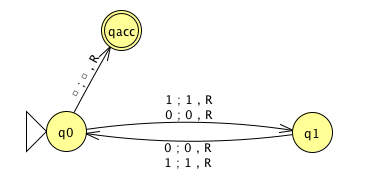
\includegraphics[width=2in]{resources/machines/Week8WarmupTM1.png} 

\columnbreak

$M_2$ 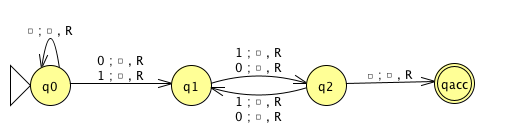
\includegraphics[width=2in]{resources/machines/Week8WarmupTM2.png}

\columnbreak

$M_3$ 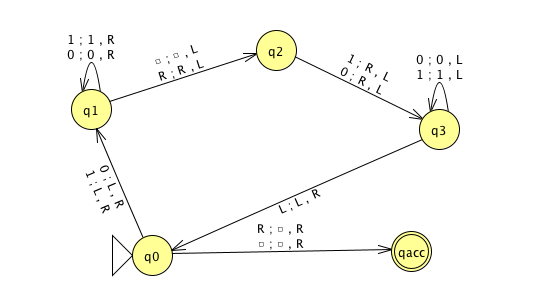
\includegraphics[width=2in]{resources/machines/Week8WarmupTM3.png}
\end{multicols}

Example strings in $A_{TM}$

\vfill

Example strings in  $E_{TM}$

\vfill

Example strings in  $EQ_{TM}$

\vfill

\newpage

{\bf  Theorem}: $A_{TM}$  is  Turing-recognizable.


{\bf  Strategy}:  To prove this theorem, we need  to  define  a Turing  machine  $R_{ATM}$ such that 
$L(R_{ATM}) = A_{TM}$.


Define $R_{ATM} =  $ ``

\vspace{150pt}


Proof of correctness: 


\vfill
\vfill

We will show that $A_{TM}$ is undecidable.   {\it First, let's explore what that means.}

\newpage

A {\bf Turing-recognizable} language is a set of strings that 
is the language recognized by some Turing machine. We also 
say that such languages are recognizable.

A {\bf Turing-decidable} language is a set of strings that 
is the language recognized by some decider. We also 
say that such languages are decidable.

An {\bf unrecognizable} language is a language that is not Turing-recognizable.

An {\bf undecidable} language is a language that is not Turing-decidable.


{\bf  True} or {\bf False}: Any  undecidable language  is  also  unrecognizable.


{\bf  True} or {\bf False}: Any  unrecognizable language  is  also  undecidable.


To prove that a computational problem is {\bf decidable}, we find/ build a Turing 
machine that recognizes the language encoding the computational problem, and that 
is a decider.


How do we prove a specific problem is {\bf not decidable}?

How would we even find such a computational problem?


{\it Counting arguments for the existence of an undecidable language:}
\begin{itemize}
    \item The set of all Turing machines is countably infinite.
    \item Each Turing-recognizable language is associated with a Turing machine
    in a one-to-one relationship, so there can be no more Turing-recognizable
    languages than there are Turing machines. 
    \item Since there are infinitely many Turing-recognizable languages
    (think of the singleton sets), there are countably infinitely 
    many Turing-recognizable languages.
    \item Such the set of Turing-decidable languages is an infinite subset 
    of the set of Turing-recognizable languages, the set of 
    Turing-decidable languages is also countably infinite.
\end{itemize}

Since there are uncountably many languages (because $\mathcal{P}(\Sigma^*)$
is uncountable), there are uncountably many unrecognizable languages
and there are uncountably many undecidable languages.


Thus, there's at least one undecidable language!

\vfill

{\bf What's a specific example of a language that is unrecognizable or undecidable?}

To prove that a language is undecidable, we need to prove that there is no Turing machine that decides it.

{\bf Key idea}: proof by contradiction relying on self-referential disagreement.

 \vfill
\end{document}